%----------------------------------------------------------------------------------------
%	SLIDE 5.
%----------------------------------------------------------------------------------------
\begin{frame}
\frametitle{An example for a parallelisable problem}
\framesubtitle{Cosmological N-body simulations}

\begin{block}{Lots and lots of similar calculations...}
	\begin{columns}
		\footnotesize
		\column{0.6\linewidth}
		\begin{equation*}
			\Psi \left( \boldsymbol{q}, \tau \right)
			=
			\int \frac{\Dcb{k}}{\left( 2 \pi \right)^{3}}
			e^{i \boldsymbol{k} * \boldsymbol{q}}
			\frac{i \boldsymbol{k}}{k^{2}}
			\delta_{L} \left( \boldsymbol{k} \right)
		\end{equation*}
		\begin{equation*}
			\boldsymbol{g}_{i}
			=
			- \nabla \phi \left( \boldsymbol{x}_{i} \right)
			=
			G
			\sum_{\mathclap{\substack{
				j \neq i \\
				j = 1
			}}}^{N} m_{j} \mathcal{F} \left( \boldsymbol{x}_{i} - \boldsymbol{x}_{j} \right)
		\end{equation*}

		\column{0.4\linewidth}
		\begin{equation*}
			\boldsymbol{x}
			=
			\boldsymbol{q} + \Psi \left( \boldsymbol{q}, \tau \right)
		\end{equation*}
		\begin{equation*}
			\dot{\boldsymbol{x}}
			=
			\frac{\dot{D} \left( a \right)}{D \left( 1 \right)} \Psi \left( \boldsymbol{q}, \tau \right)
		\end{equation*}
	\end{columns}
\end{block}

\begin{figure}
	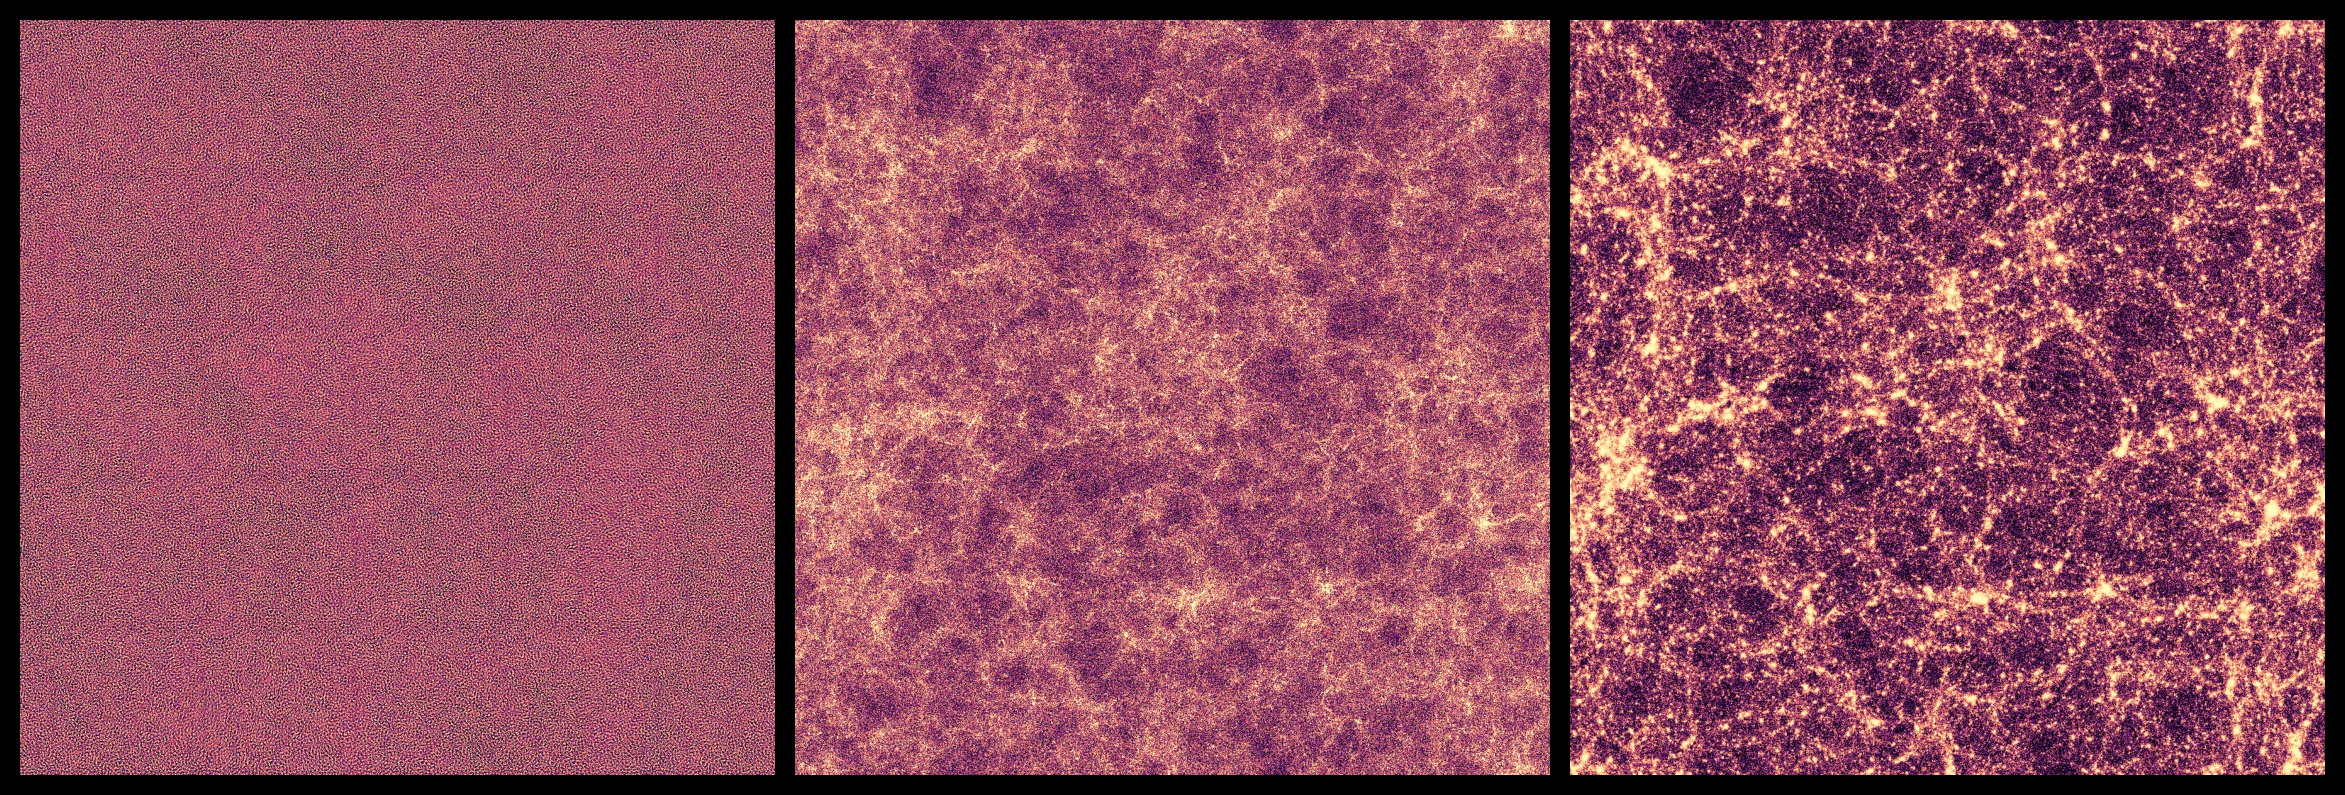
\includegraphics[width=\textwidth]{img/shaded_evolution_N65536_M2_L200_noframe.jpg}
\end{figure}

\end{frame}